\chapter[国内外相关研究综述]{国内外相关研究综述}

\section{时间序列预测研究综述}
预测建模问题是气象水文~\cite{mudelseeTrend2019},公共卫生~\cite{chimmulaTime2020},电力系统~\cite{qiuEmpirical2017}和金融市场~\cite{niuDeveloping2020}等众多领域进行管理决策时的重要问题。例如,在电力系统的运行中,电力管理部门与发电企业需要预知未来时间的区域电力负荷、火电燃煤价格、风能光伏出力等信息,从而调整电力生产与配送电计划、燃料购买与存取用计划以及电力价格定价策略等决策,以确保电网安全、稳定、经济和高效的运行~\cite{hu2015jiyu};用电企业则需要预知未来的电力价格,从而调整工业生产计划,以降低企业用能成本,维持电力交易市场的稳定\cite{hongEnergy2020}。

如果能够建立一种模型以精准描述现实现象发生的规律,如构造区域电力负荷变化规律的确定性函数,则能够正确推算出未来的状态。然而,在复杂且动态的现实背景下,管理应用领域所关注的现象往往是不确定的,比如,经济的发展、天气的变化、甚至席卷世界的COVID19疫情波动等因素都会使得电力供需发生改变\cite{heHybrid2019,liuPower2022,obstAdaptive2021}。因此,种种未知因素的存在使得难以建立完备的因果关系来给出现象发生的定律,从而不可能建立出一个确定性的模型来精确计算现象的未来表现\cite{boxTime2011}。

尽管如此,依然有可能基于对现实现象的历史观测推导出一个模型,用来计算一定提前期的未来状态。这种基于现实现象自身的历史状态建立未来状态预测模型的方法被称为时间序列预测方法。其中,时间序列是指根据时间发生的历史先后顺序得到的序列形式数据观测值。众多管理领域的核心关注数据都是以时间序列的形式存在,例如气象水文领域中的温度时间序列、公共卫生领域中的流感阳性样本率时间序列、电力系统领域中的电力负荷时间序列和金融市场领域中的股票指数时间序列,等等。这类数据的典型特征便是相邻的观测值之间存在着相互依赖性。时间序列预测正是通过对时间序列观测值之间相互依赖性的分析,发展出动态模型,进而对时间序列的未来状态进行预测。

因此,时间序列预测的本质是一个以历史时间序列输入为自变量,以未来时间序列目标为因变量的函数逼近过程。
如Hewamalage et al.~\cite{hewamalageRecurrent2021}所定义的,时间序列预测问题可以被表示为如何基于过去时刻的时间序列观测值来生成未来时刻时间序列观测值的问题,具体如下:

给定一个历史T步的时间序列向量$\bm{x} = (x_1, \ldots, x_T)$,\(\x \in \mathr^{T}\),以及未来提前H步的时间序列向量$\bm{y} = (x_{T+1},\ldots,x_{T+H})$, \(\y \in \mathr^{H}\),时间序列预测问题可被公式化定义为:
\begin{equation}
    \mathcal{F} : f(\bm x) + \bm e = \bm y. \label{eq:sec.intro.def}
\end{equation}

\autoref{eq:sec.intro.def}中,$\mathcal{F}$是指时间序列预测模型所逼近的函数。\(f\)是指时间序列预测模型所学习出的预测函数,预测函数\(f\)基于历史$T$步内的时间序列观测值,生成提前$H$步的时间序列观测值\(\hat{\y} = f(\x)\)。$T$是历史的输入步长,$H$是未来的预测时长。\(\e\)表示模型的预测误差向量:\( \e = \y - \hat{\y} \),\(\e \in \mathr^{H}\)。

时间序列预测问题作为普遍存在于不同领域中的重要问题,成为了学术界与工业界长久以来的关注焦点,受到了诸多研究者和从业者的广泛重视。针对时间序列预测问题,已发展出了众多的时间序列预测建模技术。
传统的预测建模技术主要包括以自回归(Auto-regressive,AR)模型~\cite{boxTime2011}、移动平均(Moving average,MA)模型\cite{gershenfeldFuture1993}、自回归移动平均混合(Auto-regressive moving average,ARMA)模型\cite{chuForecasting2009}、整合移动平均自回归(Auto-regressive integrated moving average,ARIMA)模型\cite{floresEvolutive2012}和指数平滑(Exponential smoothing,ES)模型~\cite{gardnerjrExponential1985,gardnerExponential2006}等以统计学为基础的时间序列预测模型。这些模型通过构造历史观测值与相关因素的经验方程,对时间序列进行拟合和预测。例如,ARMA模型通过构造当前时刻滞后一定阶数的自回归项和误差累计项的线性组合,得到提前单步的预测值。
这些传统的预测建模方法通过分析特定领域的时间序列数据特征,建立出合适的预测函数,在一些时间序列预测问题中得到了成功应用。比如,Ediger et al.~\cite{edigerARIMA2007}应用ARIMA模型对土耳其2005年至2020年间的初级能源需求量进行了预测,并在结果中展示了ARIMA模型相对人工预测方法更高的准确度。
Chu\cite{chuForecasting2009}应用ARMA模型对亚太地区的游客数量进行了预测。
Christiaanse\cite{christiaanseShortTerm1971}针对短期电力负荷预测问题建立了一种基于ES的电力负荷预测模型。

然而,这些传统的统计预测方法往往将时间序列数据的输入输出映射视为预定义的函数,因此仅适用于某一特定类型的非平稳过程,而不能有效处理复杂非线性非平稳的时间序列预测问题\cite{boxTime2011}。
基于此,非线性预测的方法和技术成为时间序列预测建模研究中的热点。
其中,基于数据驱动的机器学习方法在时间序列建模预测领域备受关注。


\section{机器学习预测建模研究综述\label{sec:ch.intro.ml}}
对于时间序列预测问题,基于机器学习(Machine learning,ML)的预测建模技术一般是将该预测问题考虑为一种以历史T步的时间序列$\bm{x} = (x_1, \ldots, x_T)$为输入,以未来提前H步的时间序列$\bm{y} = (x_{T+1},\ldots,x_{T+H})$为输出的回归问题,进而构造监督机制下的回归模型予以求解。因此,对于基于机器学习的预测建模技术而言,其拟合过程可表示为:
\begin{equation}
    f(\bm x) + \bm e = \bm y, \quad f \in \{\vartheta, \theta\}\label{eq:sec.intro.ml}.
\end{equation}

\autoref{eq:sec.intro.ml}中,\(\theta\)表示机器学习预测模型的权重参数集合,\(\vartheta\)表示定义机器学习预测模型与权重学习机制的超参数集合。这里的超参数一般指代模型中权重参数以外的参数。针对不同的模型,\(\vartheta\)具有不同的内涵。例如,支持向量机(Support vector machine, SVM)模型中的\(\vartheta\)包含了核函数(Kernel function)的类型与参数、求解输出权重时的惩罚因子、误差松弛系数等参数,神经网络(Neural Network,NN)模型的\(\vartheta\)则包含了隐藏层的层数、每个隐藏层内神经元的数量以及激活函数的类型、权重训练方法的类型及其参数,等等。

概括而言,\(\vartheta\)定义了机器学习预测模型的结构以及权重参数的训练机制,\(\theta\)表示机器学习模型从输入变换到输出间的权重参数集合。在\(\vartheta\)与\(\theta\)的联合定义下,基于机器学习建模技术的时间序列预测模型\(f\)得以确定,即\(f \in \{\vartheta, \theta\}\)。

自然地,如何选择合适的\(\vartheta\)与\(\theta\)从而建立一个精准的预测模型\(f\)以降低模型预测误差,便是时间序列机器学习预测建模技术研究所关注的核心问题。
围绕此问题,涌现了大量的模型构造方法研究与模型优化机制研究。其中,以SVM和NN为代表的机器学习模型及其优化技术在时间序列建模问题中得到了广泛研究与应用。

在此,为更好介绍基于数据驱动的时间序列机器学习预测建模技术研究,以一组给定包含\(N\)个样本的时间序列数据\(\mathbb{D} = \left\{\left(\x_{n}, \y_{n}\right) \in\left(\mathbb{R}^{T} \times \mathbb{R}^{H}\right)\right\}_{n=1}^{N}\)为例,对基于SVM与NN的预测建模技术与应用展开概述。\(\left(\x_{n}, \y_{n}\right) \)表示第\(n\)个时间序列数据输入与输出的样本对。


\begin{figure}[t!]
    \centering
    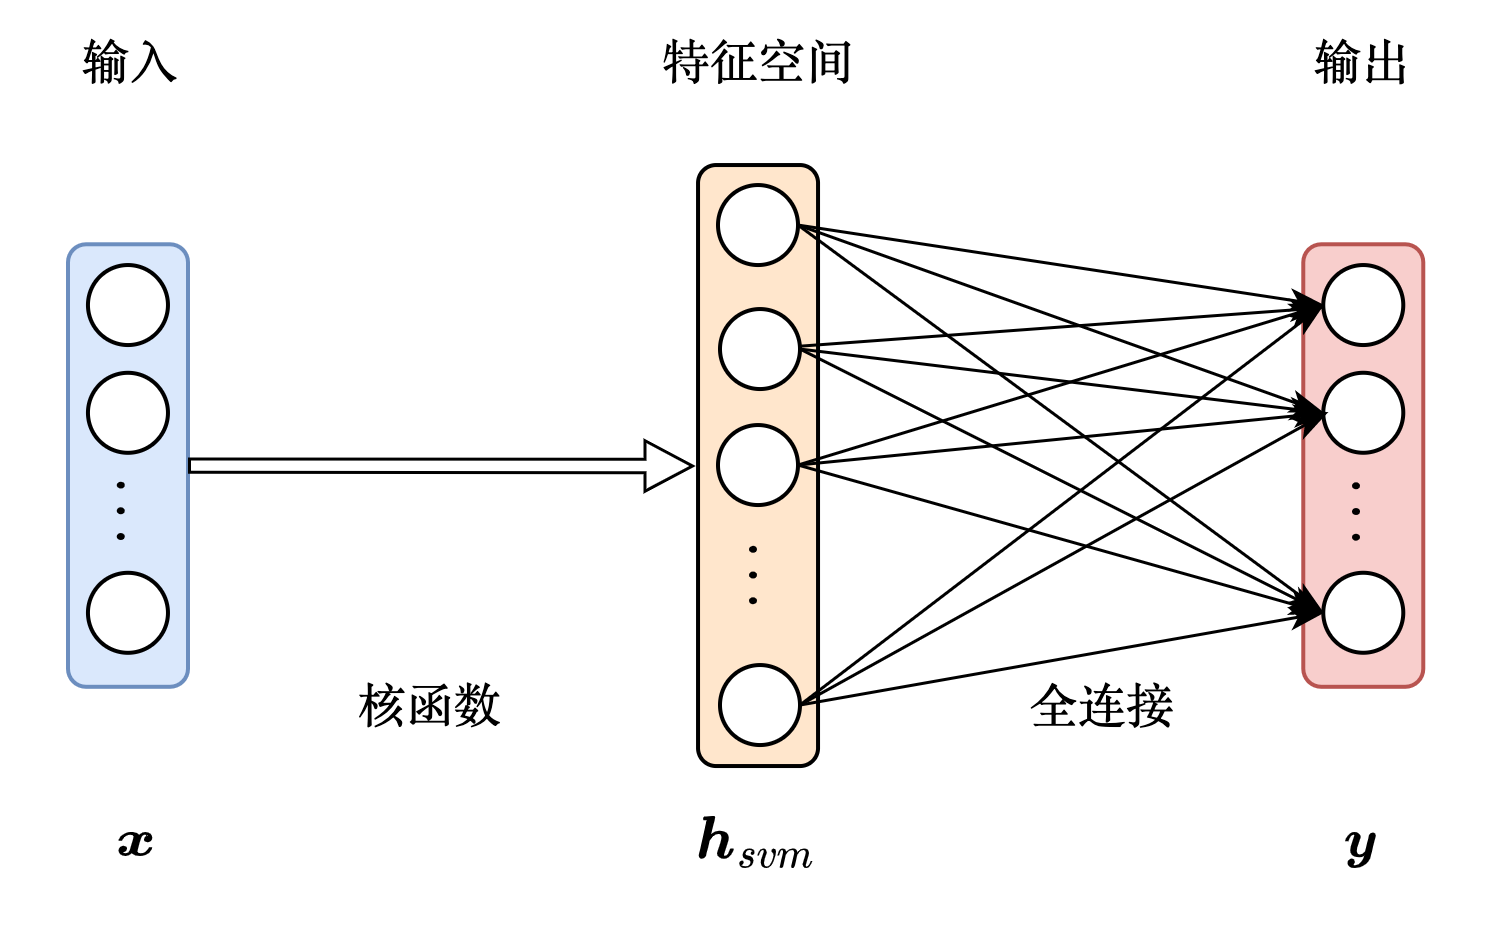
\includegraphics[width=0.8\textwidth]{float/ch.intro/svm.png}
    \caption{支持向量机结构示例\label{fig:ch.intro.svm}}
    % \setlength{\belowcaptionskip}{-10pt}
\end{figure}

\subsection{基于SVM的预测建模方法}
SVM是Vpanik~\cite{vapnikNature2013}基于统计学习理论所提出的一种机器学习方法,通过使用结构风险最小化原则代替传统的经验风险最小化原则,使其能较好解决有限样本的学习问题与过拟合问题。针对非线性不平稳的时间序列建模问题,如\autoref{fig:ch.intro.svm}所示,SVM预测模型通过引入核函数对非线性非平稳的时间序列输入特征\(\x\)进行核化,从而建立时间序列输入特征的高维特征空间表达\(\h_{svm}\),在求解输出权重时采用结合$L_2$正则化的合页损失(Hinge loss)实现结构风险最小原则,以此实现建模预测:
% \vspace{-4pt}
\begin{align}
    f_{svm}(\x) &= \w_{out}\h_{svm}, \label{eq:ch.intro.svmA} \\
    \h_{svm} &= \phi (\x)  \label{eq:ch.intro.svmC}.
\end{align}

\autoref{eq:ch.intro.svmA}中\(\w_{out}\)表示SVM预测模型的输出权重,\(\h_{svm}\)是SVM基于\autoref{eq:ch.intro.svmC}中核函数\(\phi(\cdot)\)所建立的特征空间状态表示。在经过以\(\mathd\)为训练集的核化后,\(\{\phi(\x_n)\}_{n=1}^N\)是一个维度为\(\mathr^{N\times N}\)的半正定(Positive semidefinite)矩阵,即有,\(\w_{out} \in \mathr^{H\times N}\)。
{\setlength{\abovedisplayskip}{12pt plus 3pt}
\setlength{\belowdisplayskip}{12pt plus 3pt}
\begin{equation}
    \w_{out} = \argmin_{\w_{out} }\left(\frac{\vartheta_{c}}{N}\sum^{N}_{n=1}\max(0, \left\lvert \y_n - f_{svm}(\x_n)\right\rvert  - \vartheta_{e}) + \frac{1}{2}\left\lVert \w_{out} \right\rVert^2\right)  .\label{eq:ch.intro.svmB}
\end{equation}
}

\autoref{eq:ch.intro.svmB}具体展示了SVM预测模型中\(\w_{out}\)通过$L_2$正则的合页损失予以求解的过程。\(\vartheta_{c}\)是指SVM的惩罚因子,用以调节合页损失与正则强度的平衡。\(\vartheta_{e}\)是指SVM的误差松弛系数,用以控制支持向量机的支持向量边界距离,从而增强SVM模型的鲁棒性。

显而易见,SVM预测模型中\(\w_{out}\)的求解问题是以约束条件为线性不等式组,目标函数为凸函数的问题。该问题是一个易于求解的典型二次规划问题。此外,对于时间序列数据\(\mathd\),一般\(N\)远大于\(T\)与\(H\)。由此,对于\(\{\x_n\}_{n=1}^N\)张成维度为\(N \times T\)的低维空间\(\mathbb{X} = \{\x_n\}_{n=1}^N \in \mathr^{N \times T}\)向由\(\{\y_n\}_{n=1}^N\)张成维度为\(N \times H\)的目标空间\(\mathbb{Y} = \{\y_n\}_{n=1}^N \in \mathr^{N \times H}\)的复杂非线性映射\(\mathcal{F}\)求解问题,SVM预测模型通过非线性核函数将其转变为高维特征空间\(\mathbb{H} := \{\phi(\x_n)\}_{n=1}^N \in \mathr^{N \times N}\)向低维空间\(\mathbb{Y}\)做线性映射的简单问题,同时利用\autoref{eq:ch.intro.svmB}中所展示的平衡性,具备了良好的预测性能。

因此,SVM预测模型具有高效、鲁棒、直接与参数易调整等特点,在时间序列预测建模研究中取得了广泛的关注和发展。例如,Fu et al.~\cite{fuEvolutionary2019}提出了一种基于SVM的人民币汇率预测模型;Hu et al.~\cite{huHybrid2015}针对短期电力负荷预测问题提出了一种基于SVM和混合特征提取策略的电力负荷预测模型;Tang et al.~\cite{tangNew2019}基于加权SVM提出了一种股票市场拐点预测模型;Xiong et al.~\cite{xiongCombination2015}将SVM模型与误差修正模型进行结合,提出了一种农产品价格预测模型。针对传统支持向量机的单步输出特点,面向时间序列的多步预测建模问题,Bao et al.~\cite{baoMultistepahead2014}基于传统的SVM模型提出了面向多步预测的多输出支持向量回归(Multiple-ouput support vector regression, MSVR)模型,并实验比较了传统单输出SVM模型与MSVR模型在不同多步预测策略(如迭代预测策略、直接预测策略和多输入多输出预测策略)下的性能表现。

针对时间序列预测建模任务下SVM的参数选择与模型选择问题,基于SVM收敛快,参数调整成本低等特点,Bao and Liu~\cite{baoFast2006}针对时间序列预测问题提出了一种基于快速网格搜索算法的SVM模型选择算法。在此基础上,Bao et al.~\cite{baoPSO2013}提出了基于粒子群优化(Particle swarm optimization,PSO)与模式搜索(Pattern search,PS)相结合的文化基因进化算法(Memetic algorithm,MA),并将其应用在SVM模型选择优化中。Hu et al.~\cite{huShortterm2016}利用PSO搜索SVM参数提出了一种基于PSO-SVM的预测模型。Hu et al.~\cite{huElectricity2013}提出了基于萤火虫算法(Firefly algorithm,FA)与PS算法相结合的MA算法,以此解决SVM电力负荷预测模型的模型选择问题。


\subsection{基于NN的预测建模方法\label{sec:ch.intro.nn}}
相较于SVM预测模型采用核函数方法进行非线性变换,且其输出权重具有闭式解的特点,基于神经网络的预测模型使用从输入层(Input layer)到隐藏层(Hidden layer)的非线性映射,对输入的非线性时间序列特征进行非线性变换,再由输出层(Output layer)对隐藏层表征的特征空间做线性组合进行预测输出。同时,基于神经网络的预测模型一般通过以均方误差(Mean square error,MSE)为损失函数(Loss function)的反向传播(Back propagation,BP)方式,通过梯度下降算法训练和优化神经网络各连接层(如输入层到隐藏层,隐藏层到隐藏层,隐藏层到输出层)的权重参数\(\theta\),从而实现预测建模~\cite{zhangSimulation2001}。

基于神经网络自身的结构特性,神经网络预测模型通过不同的神经网络隐藏结构构造方式以及网络权重参数训练方式衍生发展出了众多的变体。其中,多层感知机(Multilayer perceptron,MLP)作为一种以直接前馈(Feedforward)多层结构且层间均以全连接方式构造的神经网络,成为了机器学习方法下神经网络预测模型的代表结构。\autoref{fig:ch.intro.mlp}展示了一种经典的单隐藏层结构MLP模型。

\begin{figure}[t!]
    \centering
    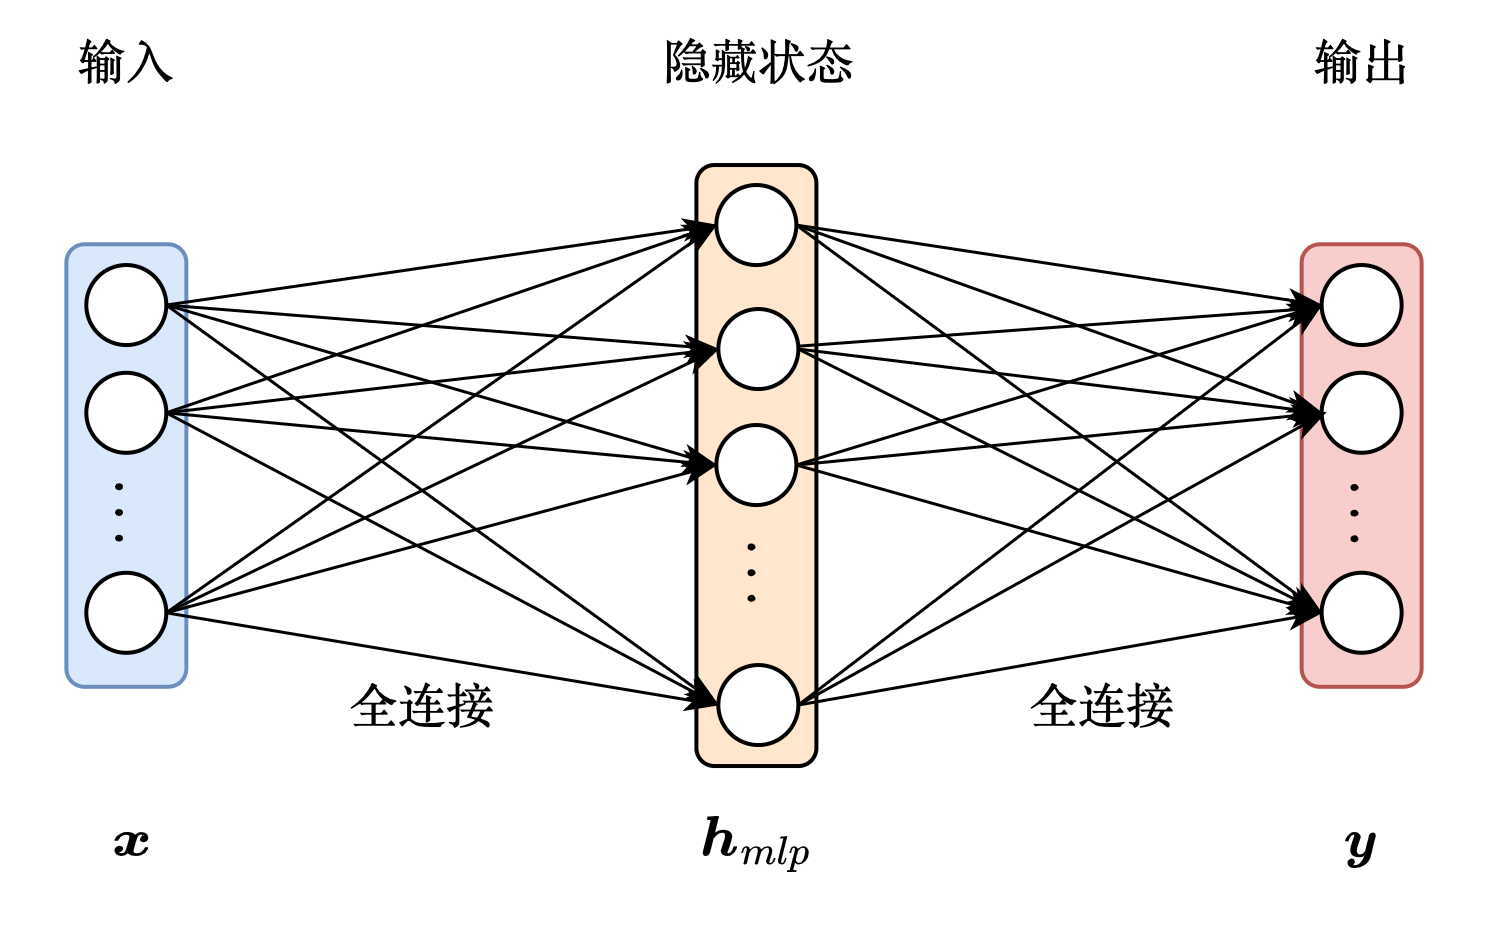
\includegraphics[width=0.8\textwidth]{float/ch.intro/mlp.png}
    \caption{多层感知机结构示例\label{fig:ch.intro.mlp}}
\end{figure}

以\autoref{fig:ch.intro.mlp}所示结构为例,其预测建模过程为:
\begin{align}
    f_{mlp}(\x) &= \w_{out}\h_{mlp}, \label{eq:ch.intro.mlpA} \\
    \h_{mlp} &= \sigma (\w_{hid}\x).  \label{eq:ch.intro.mlpB} 
\end{align}

\autoref{eq:ch.intro.mlpA}中\(\w_{out}\)同样表示模型的输出权重,\(\h_{mlp}\)是MLP通过\autoref{eq:ch.intro.mlpB}中激活函数\(\sigma(\cdot)\)对输入特征\(\x\)做非线性变换得到的隐藏层中隐藏状态状态表示。设该MLP模型中隐藏层神经元数量为\(K\),一般\(K\)大于 \(T\),远大于\(H\)。在经过训练集\(\mathd\)上的非线性变换后,使得低维输入空间\(\mathbb{X} = \{\x_n\}_{n=1}^N \in \mathr^{N \times T}\)至目标空间\(\mathbb{Y} = \{\y_n\}_{n=1}^N \in \mathr^{N \times H}\)的复杂非线性映射\(\mathcal{F}\)求解问题,通过隐藏层的非线性变换转变为高维特征空间\(\mathbb{H} := \{\sigma (\w_{hid}\x_n)\}_{n=1}^N \in \mathr^{N \times K}\)向低维空间\(\mathbb{Y}\)线性映射的简单问题。

通过对比\autoref{fig:ch.intro.mlp}与\autoref{fig:ch.intro.svm},以及对比\autoref{eq:ch.intro.mlpA}与\autoref{eq:ch.intro.svmA},可见MLP模型与SVM模型处理时间序列预测这一复杂问题的思路是一致。区别在于,SVM模型低维输入空间向高维特征空间变换是基于其\(\vartheta\)所定义的核函数,\autoref{eq:ch.intro.svmB}中输出权重的求解是闭式的;而MLP模型的特征空间变换是基于其\(\vartheta\)所定义的隐藏层结构与\(\theta\)所包含的隐藏层权重,且权重参数\(\theta:=\{\w_{out},\w_{hid}\}\)的优化问题是非凸的。

事实上,以MLP为代表,神经网络模型权重参数\(\theta\)的优化问题是普遍非凸的,且随着神经网络模型隐藏结构复杂程度的加深,例如隐藏层数的增加,而更加难以求解。针对此问题,基于反向传播(Back propagation,BP)的梯度下降(Gradient descent,GD)方法是一种有效且通行的方案。也因此,常有学者将基于梯度下降训练的神经网络模型称为反向传播神经网络(Back propagation neural network,BPNN)模型\cite{wangBack2015,wongTime1991,wangForecasting2011,dongSmall2018}。

其中,反向传播是指梯度下降训练方法中计算各层权重参数梯度时所使用的链式法则梯度传导过程。具体地,\(\theta\)的优化问题可以被视为以权重参数为自变量,以损失函数值为因变量,寻找合适的权重参数以找寻最小损失函数值的问题。设,\(\w\)表示权重参数集合\(\theta\)中的某一权重项,例如\autoref{eq:ch.intro.mlpA}中的输出层权重\(\w_{out}\)或\autoref{eq:ch.intro.mlpB}中的隐藏层权重\(\w_{hid}\),神经网络模型的损失函数为\(\ell(\w)\)。在经过以\(\mathd\)为训练集的神经网络预测模型表征后,一般有:
\begin{align}
    \ell(\w) &= \frac{1}{N \times H} \sum^N_{n=1} \|\e_{n}\| ,\label{eq:ch.intro.mse}\\
    \e_{n} & = \y_n - f(\x_n) \label{eq:ch.intro.en}.
\end{align}

\autoref{eq:ch.intro.mse}展示了神经网络预测模型在训练集\(\mathd\)上的MSE损失,其中,如\autoref{eq:ch.intro.en}所示,\(\e_n\)表示模型在训练集\(\mathd\)中第\(n\)个样本对上的预测误差向量,\(\norm{\e_n}\)是预测误差向量\(\e_n\)的$L_2$范数。

梯度下降方法的核心思想在于,基于神经网络中激活函数的连续性与可微性,通过向\(\w\)添加一个很小的动量\(\Delta_{\w}\),即\(\norm{\Delta_{\w}}\)很小,等价于\(\w + \Delta_{\w}\)近似\(\w\),利用泰勒近似将复杂非凸的\(\ell(\w)\)函数优化问题当作一个简单的函数极小值求解问题。其中,\(\ell({\w + \Delta_{\w}})\)可用一阶泰勒展开予以近似:
\begin{equation}
    \ell({\w + \Delta_{\w}} ) \approx \ell({\w}) +  \nabla_{\w}^\trans \Delta_{\w}. \label{eq:ch.intro.gd}
\end{equation}

\autoref{eq:ch.intro.gd}中,\(\nabla_{\w}\)表示\(\w\)在误差函数\(\ell\)中的梯度。此时,梯度下降方法的目标便是找寻合适的动量\(\Delta_{\w}\)使得\autoref{eq:ch.intro.gd}中损失函数\(\ell\)最小。在最陡下降中,定义学习速率(Learning rate)为\(\eta \),且\(\eta  > 0\),令:
\(\Delta_{\w} = -\eta \nabla_{\w}\)。
则有如\autoref{eq:ch.intro.eta}所示不等式性质:
\begin{equation}
\ell({\w}) > 0 \quad \text{且} \quad \eta  \nabla_{\w}^\trans \nabla_{\w} > 0. \label{eq:ch.intro.eta}
\end{equation}

当\(\eta \)足够小时,\autoref{eq:ch.intro.gd}的条件得到满足,即可直接证明出如\autoref{eq:ch.intro.lr}所示收敛性质:
\begin{equation}
    \ell({\w -\eta \nabla_{\w}} ) \approx \ell({\w})  -\eta  \nabla_{\w}^\trans \nabla_{\w} < \ell({\w}). \label{eq:ch.intro.lr}
\end{equation}


\begin{algorithm}[t!]
    \caption{神经网络模型梯度下降方法训练过程}
    \renewcommand{\algorithmcfname}{算法}
    \renewcommand{\algorithmicrequire}{\textbf{输入:}}
    \renewcommand{\algorithmicensure}{\textbf{输出:}}
    \label{alg:ch.intro.gd}
    \begin{algorithmic}[1]
        \REQUIRE {数据集\(\mathd= \left\{\left(\x_{n}, \y_{n}\right) \in\left(\mathbb{R}^{T} \times \mathbb{R}^{H}\right)\right\}_{n=1}^{N}\),神经网络模型超参数集合\(\vartheta\)
        }
        \REQUIRE {
            基于设定的神经网络模型超参数集合\(\vartheta\),初始化如下参数:\\
            梯度下降方法的当前迭代次数\(i\leftarrow 0\)\\
            当前迭代次数下神经网络权重参数集合\(\theta^i\)\\
            与模型训练相关的其他参数
        }
        \ENSURE{神经网络模型权重参数集合\(\theta\),神经网络模型超参数集合\(\vartheta\),确定神经网络模型\(f \in \{\vartheta, \theta\}\)
        }
        \WHILE{未满足\(\vartheta\)界定的收敛条件}
        \STATE \(i\leftarrow i+1\)
        \STATE 基于\(\theta^i\),确定模型\(f \leftarrow  f \in \{\vartheta, \theta^i\}\)
        \STATE 基于数据集\(\mathd\)和模型\(f\),完成前馈过程\(f(\x)\),计算模型损失函数值\(\ell({\w}) \)
        \FOR{\(\w\) in \(\theta^i\) }
        \STATE 选取计算梯度所需的样本
        \STATE 根据反向传播链式法则计算梯度信息\(\nabla_{\w}\)
        \STATE 根据梯度下降更新公式更新权重参数\(\w\)
        \ENDFOR
        \ENDWHILE
        \RETURN {
            已完成更新过程的权重参数集合\(\theta \leftarrow \theta^i\)
        }
    \end{algorithmic}
    \medskip
\end{algorithm}

同时,借助从输出层向输入层的反向传播过程,通过链式法则可以依次计算出输出端至输入端所有权重参数的局部梯度,
从而完成模型权重参数集合\(\theta\)内所有权重参数的单次更新。完整的神经网络预测模型训练过程如算法\ref{alg:ch.intro.gd}所示。

显然,梯度下降方法的性能与效率直接决定了基于梯度下降方法训练权重参数的神经网络模型性能与建模效率~\cite{liuImproved2020}。因此,神经网络梯度下降方法的改良问题成为了神经网络建模技术研究中的重要问题。围绕此问题,已发展出了众多梯度下降改进方法。
例如,基于牛顿法的梯度下降方法~\cite{bennettNewton1916}将凸优化中的牛顿法(Newton method)引入非凸的神经网络权重参数优化问题中,通过将\autoref{eq:ch.intro.gd}中的一阶泰勒近似调整为二阶泰勒近似,加速了神经网络模型的收敛速度\cite{nesterovMethod1983a,nesterovCubic2006}。
随机梯度下降(Stochastic gradient descent,SGD)方法~\cite{bottouStochastic2012}则通过将\autoref{eq:ch.intro.mse}中基于完整训练集的损失函数计算方式修改为基于随机选取的单个样本来计算损失函数值,从而大大降低了梯度下降方法的计算复杂度。
为抑制SGD方法随机选取样本所带来的梯度震荡,Sutskever et al.~\cite{sutskeverImportance2013}引入了动量(Momentum)的概念,通过向\autoref{eq:ch.intro.gd}中的梯度向量添加动量,使得模型权重参数向相关方向加速变换,从而实现加速收敛。
针对\autoref{eq:ch.intro.lr}中学习速率的选择问题,Duchi et al.~\cite{duchiAdaptive2011}提出了自适应梯度法(Adaptive gradient algorithm,AdaGrad),通过对较为密集的特征设置较小的学习速率,对较为稀疏的特征设置较大的学习速率,从而实现了针对特征的学习速率自适应设置。

% \raggedbottom
概括而言,尽管这些梯度下降方法的细节各有不同,但基于梯度下降方法的神经网络模型总体遵循算法\ref{alg:ch.intro.gd}中所示的输入、输出与执行步骤完成模型的参数优化。由此,通过梯度下降方法的权重参数训练,机器学习方法下的神经网络预测模型具备了良好的预测性能。

其中,前文所举例的MLP预测模型凭借其神经网络结构相对简单,权重参数较易训练,可通过构造具有多个神经元的输入层与输出层自然实现多输入多输出(Multiple-input Multiple-output,MIMO)策略等特点,被广泛应用于时间序列预测建模任务,尤其是提前多步预测的预测建模任务中。例如,Hamzaçebi et al.~\cite{hamzacebiComparison2009}比较了MLP在多步时间序列预测任务中采用直接策略与迭代策略的性能差异。相对于以往采用单一MLP进行多步预测的方法,Adeodato and Monteiro~\cite{adeodatoMLP2011}提出了一种基于集成思想的多步预测方法,通过集成多个MLP进行多步时间序列预测,从而提升了预测精度。
Flores et al.~\cite{floresEvolutive2012}通过遗传算法(Genetic algorithm,GA)对MLP中的隐藏层单元数、激活函数的种类进行优化,提出了一种基于GA-MLP的预测方法。
Bao et al.~\cite{baoPSOMISMO2014}针对时间序列的多步预测问题,以MLP作为预测模型,提出了一种基于PSO的多输入子多输出时间序列预测建模策略,更进一步地提升了多层感知机在时间序列多步预测上的性能。针对流感预测问题,Yang and Bao~\cite{yangComprehensive2021}通过实验表明了在多输入多输出策略、直接策略和迭代策略以及MLP预测模型和MSVR模型的策略与模型两两组合中,基于MIMO策略的MLP模型和MSVR模型具备更高的预测精度。
% \clearpage

\section{深度学习预测建模研究综述}
\subsection{深度学习建模方法}
近年来,得益于海量数据的积累、计算设备浮点运算能力的大幅提升、梯度下降方法的改进、以及通用神经网络建模框架(如Google推出的Tensorflow~\cite{abadiTensorflow2016},Meta\footnote{曾用名Facebook。Facebook于2021年10月改名为Meta。}推出的Pytorch~\cite{paszkePytorch2019}和Microsoft推出的CNTK~\cite{seideCNTK2016}等)的出现与推广,以卷积神经网络(Convolution Neural Network,CNN)~\cite{li2016juanji}和循环神经网络(Recurrent Neural Network,RNN)~\cite{yang2018xunhuan}为代表结构的深度学习(Deep learning,DL)建模技术受到了学术界和工业界的广泛关注和研究。

深度学习建模技术是机器学习建模技术中一类基于深度神经网络(Deep neural network,DNN)的建模技术\cite{lecunDeep2015}。其中,DNN是对基于不同深度神经结构所构建的神经网络的统称。例如,基于卷积结构的CNN和基于循环结构的RNN均属于DNN,其是DNN在不同特定结构上的具体实现。

深度学习建模技术与传统机器学习建模技术之间的区别在于,针对一些复杂场景的建模问题,例如计算机视觉(Computer vision,CV)中的图像分类问题\cite{dengImageNet2009}和自然语言处理(Natural language processing,NLP)中的文本分类问题\cite{maasLearning2011},传统的机器学习建模技术受限于简单的模型结构,在原始输入特征的基础上难以直接取得较好的分类结果,因此往往需要人工经验建立特定的特征提取方法,如基于图像像素数值高斯分布(Gaussian distribution)描述图像特征的Fisher Vector方法\cite{sanchezHighdimensional2011,sanchezImage2013,perronninLargescale2010}和基于语言文档内词频信息描述语句特征的词频-逆文档(Term frequency - inverse document frequency,TF-IDF)方法\cite{aizawaInformationtheoretic2003,jonesStatistical1972,luhnStatistical1957},从原始数据输入特征中提取出新的特征以提升机器学习模型处理这些问题的能力。而深度学习建模技术则直接将原始数据特征作为输入,依靠DNN的神经网络结构,如CNN中的卷积结构和RNN中的循环结构,在模型权重参数的训练中学习出数据的特征表示,成功增强了模型对于问题理解能力与解决能力。

\begin{figure}[t!]
    \centering
    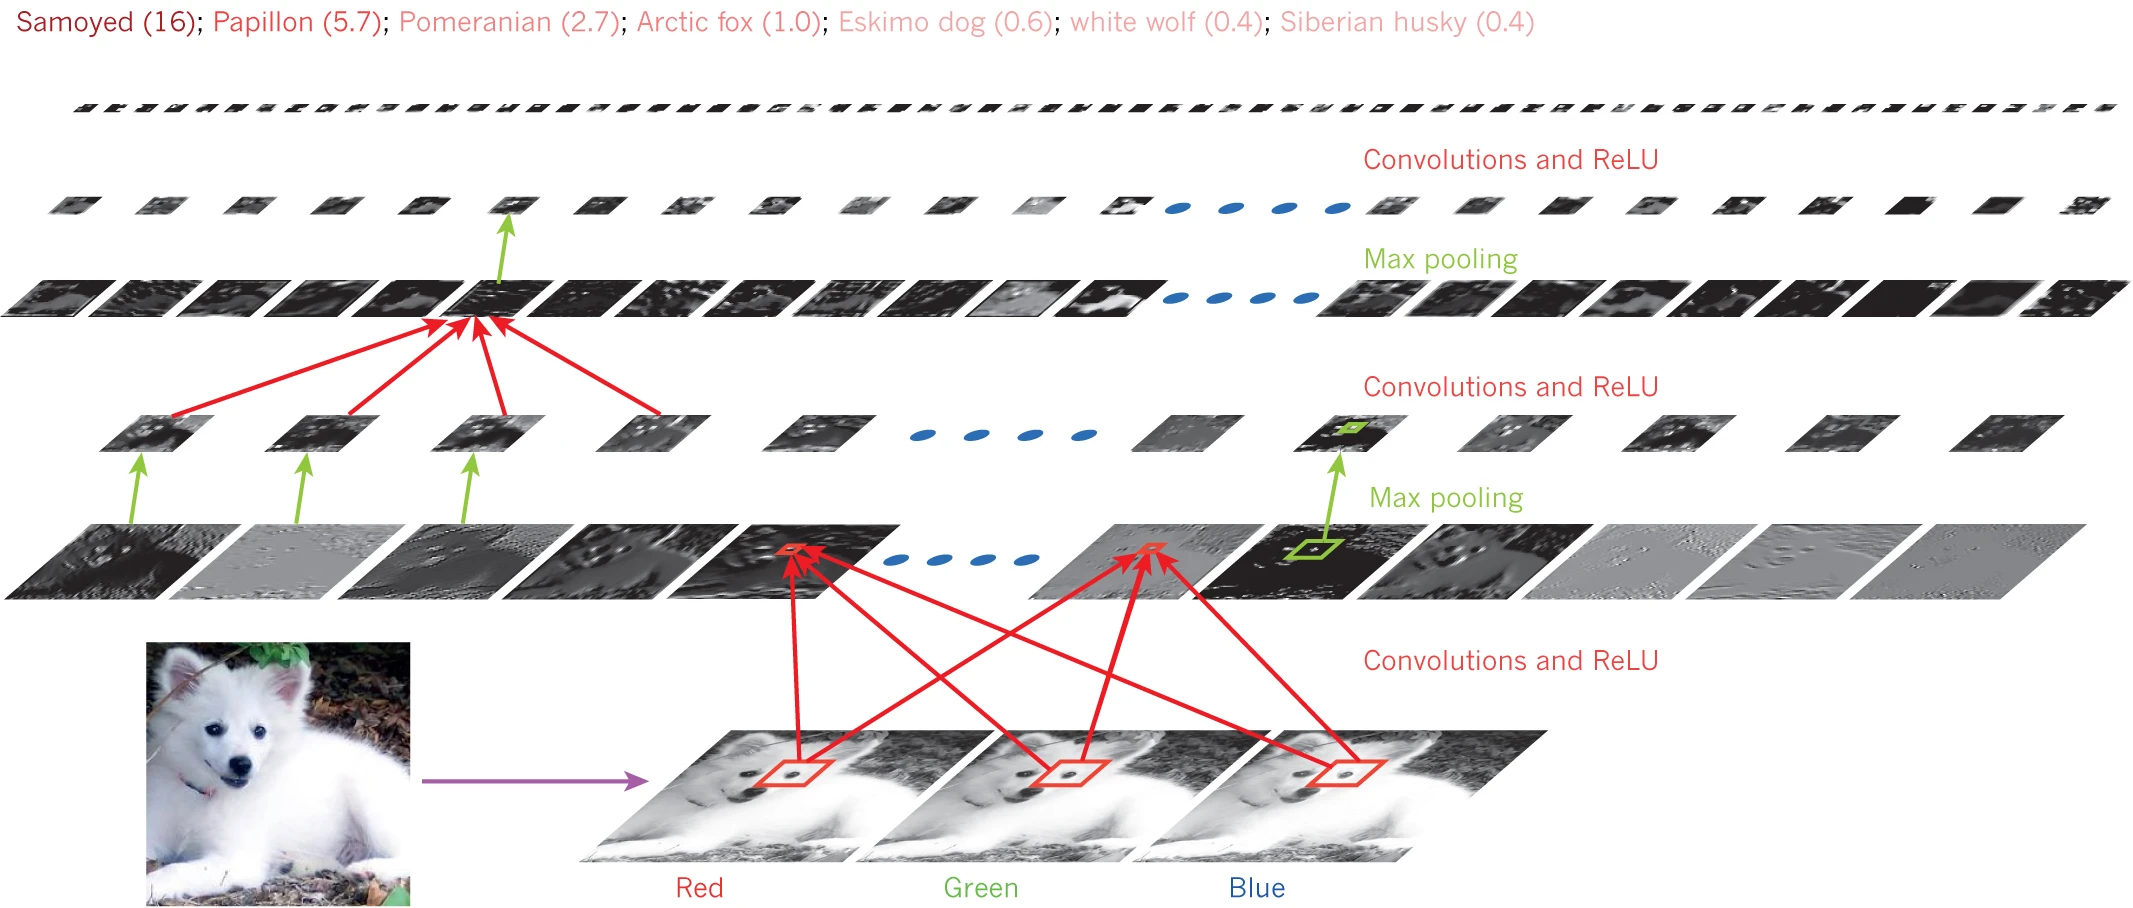
\includegraphics[width = \linewidth]{float/ch.intro/lecun.png}
    \caption{卷积神经网络图像分类模型示例(引用于Lecun et al. Deep Learning. Nature, 2015, 521(7553): 436-444,详见文献~\cite{lecunDeep2015})} 
    \label{fig:ch.intro.lecun}
\end{figure}

\autoref{fig:ch.intro.lecun}通过引用Lecun等\cite{lecunDeep2015}在Nature期刊上的CNN图像分类模型示例,形象展示了CNN基于卷积结构逐层学习图像特征表示的过程。其中,红色线表示卷积层(Convolutional layer)的卷积操作,绿色线表示池化层(Pooling layer)的下采样操作,图底处的“Red”、“Green”和“Blue”分别表示彩色图片在红绿蓝三原色下的数值状态,图顶处“Samoyed(16)”等信息展示出模型在各图片类别上的置信度,基于置信度信息,可知模型成功分类出了图片所展示的萨摩耶犬种类别。

作为在图像处理和自然语言处理等领域表现出优异性能的深度神经网络~\cite{alomStateoftheart2019},CNN与RNN在时间序列预测建模任务上的应用也成为了近年来的研究热点~\cite{sezerFinancial2020,lindbergLongterm2019,mudelseeTrend2019}。例如,Sadaei et al.~\cite{sadaei2019short}提出了一种基于CNN的短期负荷预测模型,通过将多变量的时间序列以图像的形式加以封装,使其作为输入来训练CNN预测模型,实验展示了该CNN负荷预测模型的优异性能。Salinas et al.~\cite{salinasDeepAR2020}对长短期记忆(Long-short term memory,LSTM)神经网络这一具有门控(Gate)机制的RNN加以改进,提出了一种名为深度自回归(Deep autoregression,DeepAR)的时间序列多步概率预测模型。Wang et al.~\cite{wangPhotovoltaic2019}将CNN与LSTM结合,通过LSTM对时间序列数据的长短期特征进行特征学习和表达,而后基于CNN对LSTM结构的表征在空间特征上进行学习,提出了一种长短时记忆卷积神经网络结构的深度时间序列预测模型,并结合光伏发电预测任务开展应用研究。



\subsection{模型选择问题}

\begin{algorithm}[t!]
    \caption{基于梯度下降方法的神经网络预测建模技术模型选择过程}
    \renewcommand{\algorithmcfname}{算法}
    \renewcommand{\algorithmicrequire}{\textbf{输入:}}
    \renewcommand{\algorithmicensure}{\textbf{输出:}}
    \label{alg:ch.intro.ms}
    \begin{algorithmic}[1]
        \REQUIRE {数据集\(\mathd= \left\{\left(\x_{n}, \y_{n}\right) \in\left(\mathbb{R}^{T} \times \mathbb{R}^{H}\right)\right\}_{n=1}^{N}\),神经网络模型超参数集合\(\vartheta\)的搜索空间\(\Omega\)
        }
        \REQUIRE {
            基于设定的超参数搜索空间\(\Omega\),初始化如下参数:\\
            模型选择方法的当前迭代次数\(j\leftarrow 0\)\\
            当前迭代次数下最优的神经网络超参数集合\(\vartheta^*\)\\
            当前迭代次数下最优的神经网络权重参数集合\(\theta^*\)\\
            与模型选择相关的其他参数
        }
        \ENSURE{神经网络模型权重参数集合\(\theta\),神经网络模型超参数集合\(\vartheta\),确定神经网络模型\(f \in \{\vartheta, \theta\}\)
        }
        \WHILE{未满足模型选择方法界定的收敛条件}
        \STATE \(j\leftarrow j+1\)
        \STATE 从超参数集合\(\vartheta\)的搜索空间\(\Omega\)中选择或更新出当前的超参数集合\(\vartheta^j\)
        \STATE 基于\(\vartheta^j\):\\
        \hspace{2em}执行算法\ref{alg:ch.intro.gd}所示步骤\\
        \hspace{2em}得到当前\(\vartheta^j\)试验下的权重参数集合\(\theta|\vartheta^j\)\\
        \hspace{2em}确定模型\(f \leftarrow  f \in \{\vartheta^j, \theta|\vartheta^j\}\)
        \STATE 基于数据集\(\mathd\)和模型\(f\),计算模型误差
        \STATE 基于模型误差与超参数更新方法:\\
        \hspace{2em}更新最优的神经网络超参数集合\(\vartheta^*\)\\
        \hspace{2em}更新最优的神经网络超参数集合\(\theta^* \leftarrow  \theta|\vartheta^*\)
        \ENDWHILE
        \RETURN {
            已完成更新过程的超参数集合\(\vartheta \leftarrow \vartheta^*\)与权重参数集合\(\theta \leftarrow \theta^*\)
        }
    \end{algorithmic}
\end{algorithm}
尽管深度学习预测建模技术在一些时间序列建模预测任务中表现出了优秀的学习能力,但在面对具体应用问题时,深度学习预测建模技术仍然会遇到建模技术所普遍面临的模型选择(Model selection)问题。具体地,模型选择问题是指,针对一个应用问题,如何找寻合适的模型参数以优化该模型性能的问题\cite{guyonModel2010,hastieElements2009,escalanteParticle2009}。

在本文所关注的时间序列预测问题中,如\autoref{eq:sec.intro.def}所示,对于由超参数集合\(\vartheta\)和权重参数集合\(\theta\)所定义的NN预测模型\(f\),其模型选择问题便是如何选择合适的\(\vartheta\)与\(\theta\)从而提升模型\(f\)预测性能的问题。具体地,模型选择过程如算法\ref{alg:ch.intro.ms}所示。

其中,权重参数集合\(\theta\)是基于算法\ref{alg:ch.intro.gd}所示的梯度下降训练方法予以确定。但如算法\ref{alg:ch.intro.gd}中的输入所示,权重参数集合\(\theta\)依赖于超参数集合\(\vartheta\)所定义的模型神经网络结构参数(如CNN模型中卷积层层数、卷积核宽度和卷积核数量等等)和梯度下降方法参数(如SGD方法中的学习速率、批次样本选取数量和动量惯性系数等等),不同的\(\vartheta\)必然会导致\(\theta\)的差异。因此,作为一类梯度下降方法训练的神经网络建模技术,基于DNN的深度学习预测建模技术在处理模型选择问题时同样需要遵循如算法\ref{alg:ch.intro.ms}所示的模型选择过程。

% \begin{figure}[t!]
%     \centering
%     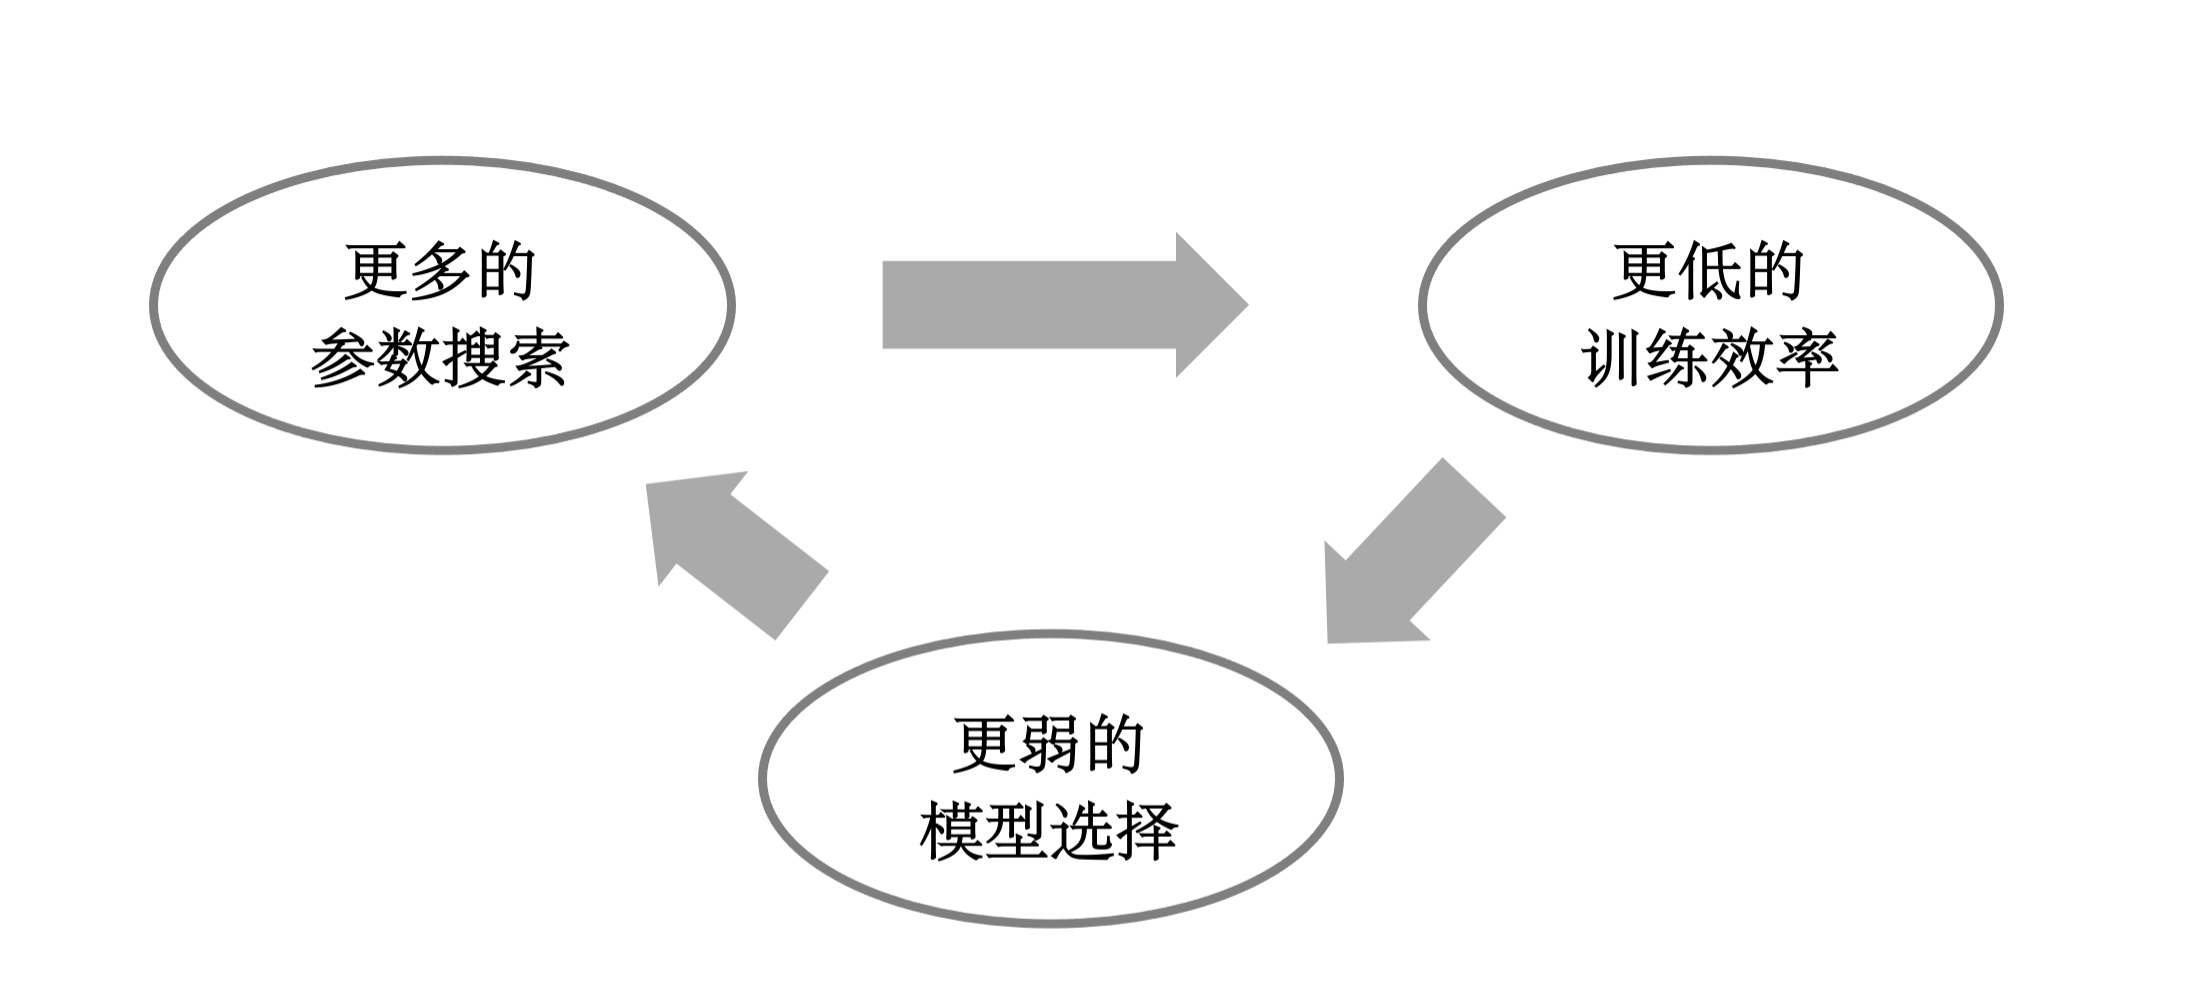
\includegraphics[width = \linewidth]{float/ch.intro/DL.png}
%     \caption{深度学习预测建模技术的模型选择挑战} 
%     \label{fig:ch.intro.dl_c}
% \end{figure}

与传统机器学习预测建模技术所遇到的模型选择挑战不同,深度学习预测建模技术所面临的模型选择挑战尤为突出。深度学习模型复杂的神经网络构型使其在实际应用时难以选择出合适的神经网络结构\cite{miikkulainenChapter2019}。这里的困难主要体现在两个方面:一是相较以MLP为代表的浅层简单结构神经网络模型,深度学习模型往往因其更深的隐藏结构而具有更多的权重参数以及更加复杂的梯度计算方式,降低了算法\ref{alg:ch.intro.ms}中步骤4所示的权重参数优化效率\cite{glorotUnderstanding2010,pascanuDifficulty2013},从而导致了深度神经网络预测建模技术模型选择效率低的问题;二是复杂的神经网络结构加深了算法\ref{alg:ch.intro.ms}中超参数搜索空间\(\Omega\)的复杂程度,从而导致了深度神经网络预测建模技术神经网络结构选择效果差的问题。尤其,
% 如\autoref{fig:ch.intro.dl_c}所示,
较低的权重参数优化效率会再次增加神经网络结构选择的难度,神经网络结构难度的加大会进一步降低模型选择的效率。


因此,在本文所聚焦的时间序列预测建模问题中,深度学习预测建模技术梯度下降方法效率低、神经网络结构复杂所导致的模型选择效果差的问题使得当前时间序列深度学习预测建模技术应用存在较大局限。这些问题大大增加了优化时间序列深度学习预测模型所需的计算时间、计算资源和人员精力,使得现实任务中的深度学习预测模型难以被精细优化,进一步限制了时间序列深度学习预测模型的准确性、稳定性、可靠性和应用性。其中,梯度下降方法是造成深度学习预测建模技术模型选择效率低下的主要因素。尽管已有众多提高梯度下降过程效率的方法\cite{bottouStochastic2012,duchiAdaptive2011,liuImproved2020},但如\autoref{sec:ch.intro.ml}中所述,这些方法仍需遵循算法\ref{alg:ch.intro.gd}中所示步骤,多次迭代计算梯度以渐进优化权重参数的本质没有改变。因此,基于梯度下降方法的深度学习预测建模技术从根源上便存在模型选择效率低的问题,在改变试验超参数时始终需要重新训练权重参数才可得到当前超参数的模型效果,其模型选择的效率难以显著降低。因而,现有的时间序列深度学习预测建模技术模型选择研究多集中于神经网络结构选择问题的研究。


时间序列深度学习预测技术中的神经网络结构选择问题是指,根据时间序列预测任务的场景如何选择合适的深度神经网络结构以实现更优的预测性能。
根据深度学习模型预测建模过程的阶段可以将神经网络结构选择问题分解为深度学习模型的表征结构选择问题与输出结构选择问题。
时间序列深度学习预测模型表征结构与输出结构分别是指深度学习模型对时间序列数据输入特征进行深层非线性表征的神经网络结构,以及对深层非线性表征结果进行解码以生成输出结果的神经网络结构。
前者具体如,CNN的输入层(Input layer)、卷积层(Convolutional layer)与池化层(Pooling layer)结构~\cite{koprinskaConvolutional2018},RNN的输入层和隐藏层(Hidden layer)结构~\cite{salinasDeepAR2020}等;而后者具体如,基于全连接层(Fully connected layer)的解码器结构~\cite{koprinskaConvolutional2018,caiDayahead2019},基于循环结构的解码器结构~\cite{liuDSTPRNN2020}
和自回归结构~\cite{caiDayahead2019,salinasDeepAR2020}等。其中,CNN预测模型因其神经网络结构的前馈机制,一般采用全连接解码器结构作为其输出结构;而RNN预测模型因其神经网络的循环机制,衍生出包括全连接结构解码器、循环结构解码器和自回归结构在内的多种输出结构。因此,表征结构的选择问题是CNN预测建模技术与RNN预测建模技术的共性问题,而输出结构的选择问题是基于RNN建模技术的深度学习预测模型特有问题。同时,RNN预测建模技术可通过调整解码器结构自然地实现不同的多输出生成策略。因此,对于基于RNN的DNN预测模型而言,时间序列预测中的多输出选择问题是其神经网络结构选择问题中的一类特定问题,表现为输出结构的选择问题。

此外,深度学习模型的表征结构可进一步细分为输入结构与隐藏结构。对基于神经网络的预测建模技术而言,因其输出层单元与时间序列多输入特征的一一对应,神经网络预测建模技术输入结构的选择直接反映了输入特征的选择。例如,Sezer and Ozbayoglu~\cite{sezer2018algorithmic}利用CNN卷积核的多通道输入能力,将金融时间序列转换为二维输入结构,以此构造基于CNN的算法交易模型。Yang et al.~\cite{yangShortterm2021}借助扩充RNN的输入层结构将传统的单变量时间序列预测建模多输入策略加以优化,使其从传统的单个输入时步对应单个输入观测值扩充为了单个输入时步对应连续多个输入观测值,通过PSO算法优化输入步长进一步提高了RNN预测模型的准确率。因此,DNN预测建模技术的特征选择问题亦可视为其神经网络结构选择问题中的一类特定问题,表现为输入结构的选择问题。

基于对时间序列深度学习预测技术神经网络结构选择问题的上述分析,加之隐藏结构在深度神经网络中权重参数与结构参数占比最多,其结构选择问题是当前神经网络结构选择问题的研究重点,本节将对神经网络隐藏结构的选择研究予以重点介绍,并将输出结构选择研究和多输出选择研究予以合并介绍,输入结构选择研究与特征选择研究亦合并介绍。

\subsubsection{DNN隐藏结构选择}
针对神经网络隐藏结构选择这一跨应用领域的共性关键建模技术问题,国内外学者展开了大量的研究与实践工作,并在一些领域率先取得了成效。这一问题的研究途径主要是将神经网络结构选择问题视为神经网络结构搜索(Neural architecture search,NAS)问题。Elsken et al.~\cite{elskenNeural2019a}针对该问题总结出搜索空间、搜索策略和性能评价三个要素,即将一系列不同的神经网络隐藏结构作为候选单元组成搜索空间,在既定的搜索空间或是自适应增长的搜索空间内,通过启发式搜索算法或强化学习算法等智能优化与搜索技术建立搜索策略寻找适应问题的最优神经网络隐藏结构,并对每一次的更新结构重新训练以做出评价。例如,Baker et al.~\cite{bakerDesigning2017}面向图像分类问题提出了一种基于强化学习的NAS方法,通过逐层的搜索和构造CNN的卷积与池化结构,从而在CIFAR-10~\footnote{图像分类领域内的基准数据集之一,共有10个类别,包含50000个训练样本与10000个测试样本。}任务上取得了优异成绩。
此外,基于Baker et al.~\cite{bakerDesigning2017}的工作,Liu et al.~\cite{liuHierarchical2018a}提出了一种基于遗传进化算法的层级NAS策略,将层级的卷积结构或池化结构作为CNN神经网络隐藏结构的候选单元个体,通过遗传进化算法的融合和变异等动作自适应地构造了分类任务下的CNN神经网络隐藏结构,并刷新了CIFAR-10任务分类准确率的历史(截至其论文发表时)最好成绩。

针对时间序列深度学习预测建模中的神经网络结构选择研究,现有研究亦关注于隐藏结构参数选择问题。Bouktif et al.~\cite{bouktifOptimal2018}针对电力负荷预测情景提出了一种基于遗传(Genetic)算法的输入特征选择与网络层数选择的LSTM时间序列预测模型,通过将既定步长的时间序列输入时步进行$\left[0,1\right]$编码,以及将LSTM隐藏层网络层数参数离散编码,以此作为基因个体代入LSTM模型中迭代训练和评价,以此对电力负荷输入数据和LSTM神经网络的隐藏层层数进行选择。
Peng et al.~\cite{pengEffective2018}针对电力价格预测任务提出了一种基于差分进化(Differential Evolution,DE)算法的LSTM预测模型选择算法。作者以固定隐藏层层数参数的LSTM神经网络作为预测模型,通过将不同输入步长,不同最大训练次数和不同隐藏层神经元个数向量化编码作为DE算法的种群个体,以此优化预测模型的输入步长和隐藏层单元数,从而提升模型预测性能。
在Bouktif et al.~\cite{bouktifOptimal2018}和Peng et al.~\cite{pengEffective2018}的研究基础上,Peng et al.~\cite{pengEffective2020}针对能源月度消耗量预测等场景,以固定隐藏层层数的LSTM作为预测模型,基于果蝇优化(Fruit fly optimization)算法对LSTM的输入步长、训练次数、隐藏层神经元个数和每批次训练样本数(Batch size)一同进行优化,以此进行参数选择。
Li et al.~\cite{liAutoST2020}针对交通流量预测情景提出了一种构造式的CNN预测模型。作者将不同的卷积结构或池化结构封装成候选单元,人工定义了不同的单元组合方式作为构造神经网络结构的动作,并建立一个独立的神经网络对动作适应性加以评估,以此解决CNN预测模型的隐藏结构选择问题。

然而,这些通过不断训练不同结构的深度学习模型来解决模型选择问题的方式意味着很高的建模复杂度、极长的优化时间和不菲的计算资源。例如,Baker et al.~
\cite{bakerDesigning2017}在CIFAR10任务的模型选择工作消耗了10张NVIDIA显卡8-10天的算力。Li et al.~\cite{liAutoST2020}需5.1小时完成北京交通流量数据集(30分钟级,共15072个观测点)上的模型选择工作。
因此,本文将针对找寻合适方法,探求高效稳定的时间序列深度学习预测模型隐藏结构构造理论与选择策略。
% \clearpage

\subsubsection{DNN输出策略选择}
深度学习预测建模技术也面临着多输出策略选择问题。由于时间序列预测任务的多输出变量与输入变量之间同样存在着复杂的关联性,且随着预测步长的增加,可能出现预测误差累计等问题\cite{sorjamaaMethodology2007}。因此针对时间序列的提前多步预测问题,需要深度学习预测模型选择合适的多输出策略。
既有多步预测策略主要包括:直接策略、迭代策略~\cite{sorjamaaMethodology2007}和MIMO策略~\cite{bontempiLong2008}。

直接策略是指对于提前多步预测任务,直接针对每个提前时步单独构造预测建模完成对应提前时步预测。
迭代策略是通过构造基于完整的多输入和提前单步观测值的组合训练出单步预测模型,而后将最早时步的输入观测值去除,将上步提前单步预测值新增进输入中,以此得到当前提前单步预测值,迭代此过程直至得到所有提前时步的预测结果。
MIMO策略则是通过构造基于完整的多输入和提前多步观测值的组合训练得到多输出预测模型。
这三种预测策略中,直接策略在破坏了输入与输出的时序连续性的同时增加了建模任务的计算开销,迭代策略则因采用无法避免误差的预测值代替真实值生成下步预测值的做法,易使预测误差随预测步长的增加显著扩大。
相比之下,MIMO策略这种构造完整的多输入多输出关系的方法能够在一定程度上解决迭代策略多步预测任务中的误差累积问题~\cite{baoPSOMISMO2014},同时避免了直接策略构造多个模型所带来的额外计算开销。

因此,现有的时间序列深度学习预测建模技术普遍采用MIMO策略构造多步预测模型~\cite{hewamalageRecurrent2021}。
如,Wu et al.~\cite{wuImproved2019}提出了一种基于经验模态分解的LSTM原油价格预测模型,结合MIMO策略进行了多步预测。
Niu et al.~\cite{niuWind2020}基于MIMO策略建立了一种基于注意力机制的GRU风力预测模型。
Masum et al.\cite{masumInvestigation2019}针对水压时间序列预测问题,比较研究了LSTM和双向LSTM(Bidirectional long short term memory,BI-LSTM)预测模型直接策略、迭代策略和MIMO策略下的表现,实验发现LSTM和BI-LSTM模型在MIMO策略下预测性能更为优异。

由于深度学习预测建模技术的灵活性,即使是在MIMO策略下,深度学习模型依然存在多种不同的多输出生成策略。Hewamalage et al.~\cite{hewamalageRecurrent2021}归纳出了RNN预测模型在MIMO预测策略下基于堆栈结构、全连接解码结构和循环解码结构的输出结构。Salinas et al.~\cite{salinasDeepAR2020}在循环解码结构的基础上,通过将编码器中的循环神经网络复用为解码器展示了一种自回归结构的多输出生成策略。
但这些研究较为简单,未有关注输出结构的选择与优化问题。
基于这样的研究背景,深度学习预测模型在时间序列多步预测任务下的输出结构选择研究仍有待补充和完善,从而建立合适的多输出生成策略,进一步提高预测模型的多步预测性能。


\subsubsection{DNN输入特征选择}

目前,已有较多研究关注了深度学习预测模型多输入的特征选择(Feature selection)问题~\cite{gaoShortTerm2019,wangNovel2020,niuDeveloping2020}。
特征选择是指从已知的输入特征候选集中,按照一定的标准,通过删除一些弱相关的输入特征以寻找出最优输入特征子集,进而降低输入特征空间的维度来改善预测模型性能的方法。

根据是否依赖预测模型的不同,可以将常用的特征选择方法分为过滤法(Filter)和封装法(Wrapper)。过滤法是一种依靠独立于预测模型的统计量来评估多输入特征与输出目标间关系的方法,而封装法是指直接通过预测模型在特征子集上预测性能表现选择特征的方法。
例如,Bouktif et al.~\cite{bouktifOptimal2018}基于封装法对电力负荷LSTM预测模型的输入特征进行挑选。 Wang et al.~\cite{wangNovel2020}利用相关特征算法对输入特征进行挑选后,再将特征子集送入RNN预测模型来对风力进行预测。基于Wang et al.~\cite{wangRandom2018}所构造的电力负荷随机森林预测模型,Zahid et al.~\cite{zahidElectricity2019}提出了一种混合过滤法和封装法的特征选择算法,首先通过递归特征消除法对电力负荷输入数据进行初步筛选,而后利用随机森林完成最终的特征选择,最终构造出基于特征选择CNN的电力负荷预测模型。
Niu et al.~\cite{niuDeveloping2020}提出了一个两阶段特征选择的深度学习预测框架,作者先通过相关特征算法对输入特征进行初筛后,再将初筛后的特征以封装法的方式送入ELM预测模型中完成第二次特征选择,最后将选择后的特征子集送入由卷积长短时记忆(Convolutional long short term memory,CLSTM)网络、LSTM网络、控制循环单元(Gated recurrent unit,GRU)网络组成的复杂网络中进行学习和训练,从而完成预测建模。

对比过滤法和封装法,已有研究表明封装法能够更有效地提升模型预测性能\cite{huHybrid2015}。
鉴于封装法下特征选择提升预测模型准确度的有效性,目前已有众多学者提出了基于封装法的多输入特征选择方法\cite{renMultivariate2022,naModified2022,wangRandom2018,yangComprehensive2021}。
例如,
Yang et al.\cite{yangComprehensive2021}等借助二元粒子群优化算法(Binary particle swarm optimization,BPSO)对以\(0,1\)二元变量编码的多输入特征和模型结构参数进行筛选,提出了一种流感阳性样本率预测的综合学习粒子群优化建模框架。

然而,深度学习建模技术兼容处理每一输入时步内多维特征的性质,如CNN卷积核的多通道性质,RNN的时步多维输入性质,使得深度学习预测建模技术的多输入选择问题不仅包含特征选择问题,也包含特征结构选择(Feature structure selection)问题。
这里的特征结构选择是指,从已知的输入时间序列特征中,通过折叠或展开相关的输入特征到对应输入时步中以寻找出最优输入特征结构,进而改善深度学习预测模型性能。
例如,Bandara et al.\cite{bandaraForecasting2020}利用RNN循环读取每一时步输入的机制,通过滑动窗口方法(Moving window schema)将单变量时间序列数据在每个时步折叠出窗口范围的连续特征,增强了RNN预测模型的准确性。Yang et al.~\cite{yangShortterm2021}针对华中地区的电力负荷预测问题,借助RNN的递归多维输入性质,通过将每条样本中时间粒度为小时的7天电力负荷输入样本数据,展开为每一输入步长包含一小时负荷值的输入结构或折叠为每一输入步长包含一天负荷值的输入结构,从而更好的建模这种内在关联性,进一步提高预测准确度。Wang et al.~\cite{wangTraffic2016}利用CNN卷积层卷积核的多通道输入性质,将每条样本中的一维道路流量时间序列折叠为二维矩阵,从而提升了CNN预测模型对于时空特征的提取学习能力。

通过上述研究与分析,基于过滤法的多输入选择方法并不完全适用于深度学习模型下的多输入特征结构选择问题,而基于封装法下的特征选择研究在深度学习建模背景下的多输入特征结构选择问题关注较少。
同时,基于封装法下的深度学习预测模型特征选择算法同样面临由于反复多次完备训练以评估特征子集而导致的计算开销高昂,效率低下等问题。
因此,本文将继续深入研究时间序列深度学习预测建模多输入选择问题,探索和发展高效优化深度学习预测模型多输入特征结构的方式方法。


\section{随机映射方法研究综述}
\subsection{基于SMLP的预测建模方法}


对于深度学习预测建模技术模型选择问题,不论是隐藏结构的及参数选择,或是输出策略与结构的选择,还是输入特征结构的选择,都受限于梯度下降方法所导致的低效性,难以在有限时间内有效解决模型选择问题,从而无法高效提升模型预测性能。针对此不足,随机映射方法是一种替代梯度下降构造深度学习预测模型的可行方法。

随机映射是最早由Schmidt et al.~\cite{schmidt1992feed}提出的一种采用非迭代学习机制的MLP建模方法。这种方法利用随机初始化,固定神经网络的输入与隐藏层权重,而后基于有监督的反馈闭式地求解神经网络输出层权重的思路建立神经网络模型,具有具备很低的计算开销、很高的学习效率与良好的非线性表达能力等优势和特点,已发展出随机向量函数链接网络(Random Vector Functional Link Network,RVFL)、极限学习机(Extreme Learning Machine,ELM)等成熟有效的随机多层感知机(Stochastic multiple percentage, SMLP)学习技术~\cite{scardapaneRandomness2017,caoReview2018,tanakaRecent2019}。

\begin{figure}[!t]
    \begin{subfigure}[b]{0.25\textwidth}
        \includegraphics[height=\linewidth]{float/ch.cnn/layer.pdf}
        \caption*{}
    \end{subfigure}
    \hspace*{-0.15\textwidth}
    \begin{subfigure}[b]{0.25\textwidth}
        \includegraphics[height=\linewidth]{float/ch.cnn/schmidt.pdf}
        \caption{Schimidt网络}
    \end{subfigure}
    \hspace*{0.03\textwidth}
    \begin{subfigure}[b]{0.25\textwidth}
        \includegraphics[height=\linewidth]{float/ch.cnn/rvfl.pdf}
        \caption{RVFL网络}
    \end{subfigure}
    \hspace*{\fill}
    \begin{subfigure}[b]{0.25\textwidth}
        \includegraphics[height=\linewidth]{float/ch.cnn/elm.pdf}
        \caption{ELM网络}
    \end{subfigure}
    \caption{\label{fig:randomnet}随机多层感知机模型示例}
\end{figure}

\autoref{fig:randomnet}展示了以Schimidt网络、RVFL网络和ELM网络为代表的SMLP模型。
以\autoref{eq:ch.intro.mlpA}和\autoref{eq:ch.intro.mlpB}及其参数定义为例,SMLP模型的预测过程如\autoref{eq:ch.intro.smlp}和\autoref{eq:ch.intro.smlp.h}所示:
\begin{align}
    f_{smlp}(\x) &= \w_{out}\h_{smlp}, \label{eq:ch.intro.smlp}\\
    \h_{smlp} &= \sigma (\w_{hid}\x). \label{eq:ch.intro.smlp.h}
\end{align}

以最小二乘法为例,\autoref{eq:ch.intro.lsq}展示了SMLP模型输出层权重\(\w_{out}\)的计算过程。其模型损失函数依然保持\autoref{eq:ch.intro.mse}所展示的MSE损失形式:
\begin{align}
    \w_{out} &= \argmin_{\w_{out}} \norm{\y - \w_{out}\h_{smlp}} \label{eq:ch.intro.lsq}\\ 
    & = \y \h_{smlp}^{\trans} (\h_{smlp}\h_{smlp}^\trans)^{-1}. \notag
\end{align}


与梯度下降方法迭代训练输出层权重\(\w_{out}\)与隐藏层权重\(\w_{hid}\)不同,随机映射方法在以一随机分布初始化隐藏层权重\(\w_{hid}\)后,固定\(\w_{hid}\),而后基于最小二乘法(Least square method)和岭回归(Ridge regression)等闭式求解方法直接计算输出层权重\(\w_{out}\)。
联系\autoref{sec:ch.intro.ml}中所述的SVN预测建模方法,对于一个确定核函数与训练数据\(\mathd\)的SVM模型,其高维特征空间\(\mathbb{H}\)与输入空间\(\mathbb{X}\)是固定的,意味着输入空间与特征空间之间存在一个确定且固定的非线性矩阵变换(即隐藏权重),且如\autoref{eq:ch.intro.svmB}所示,SVM模型的输出权重求解方法同样是闭式求解方法。
因此,\autoref{sec:ch.intro.ml}中所述的支持向量机模型是一种SMLP模型的特例\cite{vapnikNature2013}。由此可见,相比于算法\ref{alg:ch.intro.gd}所描述的迭代式梯度下降权重参数训练方法,随机映射方法通过单次模型前馈过程即可完成整个模型的权重参数训练,极大提高了模型构造效率。

虽然传统的SMLP模型避免了梯度下降训练计算开销高的问题,但这种权重随机机制使其模型性能的收敛性与稳定性受到质疑。针对于此,Huang et al.~\cite{huang2006universal}基于递归添加神经元的方式构造了一种增长极限感知机(Incremental extreme learning machine,IELM),并证明了IELM对于任意连续有界目标函数的学习收敛能力。
在此基础上,Wang and Li\cite{wang2017stochastic}提出了一种随机配置网络(Stochastic configuration network,SCN),通过迭代增加隐藏层神经元,基于监督机制闭式挑选神经元隐藏层权重,全局更新输出层权重的方式,构造出增长的SMLP模型,并证明了SCN的普适逼近性质(Universal approximation property)。基于此,通过改进模型神经网络构造方法,所建立的SMLP模型可具有理论保证的拟合收敛性与稳定性。

目前,国内外学者基于SMLP模型展开了广泛的时间序列预测建模技术与应用研究。如,Xue et al.~\cite{xueFinancial2018}提出了一种基于ELM和正则化方法的现金流预测模型。Xiong et al.~\cite{xiongSeasonal2018}利用ELM和季节趋势分解技术建立了一种农产品价格时间序列预测模型。利用RVFL收敛速度快,建模效率高的优势,Yu et al.~\cite{yuInvestigation2020}集成了多个不同参数设置的RVFL,构造集成模型进行原油价格预测。基于分类问题下ELM在深层神经网络结构方向上的探索和尝试~\cite{yuLearning2015,tangExtreme2016},Song et al.~\cite{songNovel2017}建立了一种集成ELM的时序序列预测建模型,作者使用了90个改进型ELM作为集成预测模型中的预测单元,在Marckey-Glass时间序列数据集~\footnote{https://en.wikipedia.org/wiki/Mackey-Glass\_equations}、St. Louis Fed金融指数时间序列数据集~\footnote{https://www.stlouisfed.org/news-releases}和太阳黑子时间序列时间数据集~\footnote{http://www.sidc.be/silso/home}上进行了测试,展示与分析了集成多层ELM的性能优越性和建模高效性。

\subsection{基于SDNN的预测建模方法}

与此同时,一系列基于随机映射方法的深度学习建模技术不断被探索和研究。
为解决RNN权重参数训练开销大,收敛速度慢等问题,Jaeger~\cite{jaegerEcho2001}于2001年基于随机映射方法提出了基于随机映射的RNN模型,并将其命名为状态回声网络(Echo state network,ESN)。作为文献中最早提出与最具代表性的随机深度神经网络(Stochastic deep neural network,SDNN)建模技术,ESN在传统RNN的基础上,基于随机映射方法将RNN中的输入层与隐藏层权重随机初始化并固定,通过最小二乘法、岭回归($L_2$正则化的最小二乘法)等闭式求解算法计算出输出层权重~\cite{shen2018duoxishu}。
这种神经网络继承了RNN序列建模的特点,能够有效的建立时间序列多输入与输出间的非线性关系,同时发挥了随机映射非迭代式训练的快速收敛优势~\cite{jaegerAdaptive2002},在时间序列预测建模领域中得到了广泛的应用和发展。
例如,Deihimi and Showkati~\cite{deihimiApplication2012}针对短期电力负荷预测问题提出了一种基于ESN的预测模型。Hu et al.~\cite{huForecasting2020}通过加深ESN的隐藏层结构,提出了一种深度的ESN时间序列预测建模,并在电力需求预测任务和风力预测任务中进行了应用研究。

针对ESN预测模型的参数选择问题,Chouikhi et al.~\cite{chouikhiPSObased2017}利用PSO对ESN预测模型的随机化权重进行训练与优化,从而提升ESN预测模型的预测性能。
在此基础上,Li et al.~\cite{liPSObased2019}建立了一个多循环池结构的ESN预测模型,通过PSO和奇异值分解对循环池权重进行训练和优化后再依次将其加入ESN网络结构中,以此进一步提升ESN的预测表现。
此外,由于ESN模型的内在随机机制,ESN预测模型的神经网络结构成为了影响其预测性能的重要因素。


针对ESN预测模型的神经网络结构构造问题,众多研究者进行了相关研究。例如,Xue et al.~\cite{xueDecoupled2007}发现ESN网络隐藏层神经元的紧密耦合使得,使得模型无法较好学习出不同尺度的时间序列特征。针对此问题,Luko{\v s}evi{\v c}ius et al.\cite{lukovsevivcius2009reservoir}将ESN网络的隐藏层分割成多个子网络,降低了隐藏层神经元间的耦合效应(Coupling effect)。基于Xue et al.~\cite{xueDecoupled2007}的工作,Qiao et al.~\cite{qiaoGrowing2017}通过向ESN隐藏层中递归添加子网络的方式逐渐加宽其隐藏结构,同时利用最小二乘法全局更新网络输出层权重,构造出生长回声状态网络(Growing echo state network,GESN)预测模型,解决了多子网络ESN模型隐藏层结构的设计问题。
但随着隐藏层的不断加宽,全局更新输出权重的加宽构造方法会显著增大输出权重计算时出现病态问题的可能性,从而破坏模型的拟合能力与预测稳定性\cite{yangDynamical2019}。
为解决此问题,Yang et al.\cite{yangDynamical2019}通过向GESN输出权重计算中的最小二乘方法加入$L_2$正则项,以岭回归的闭式计算方法求解GESN输出权重。
Li et al.\cite{liPSObased2019} 通过引入GESN迭代构造过程中的预测误差反馈,基于迭代局部更新的方式降低了输出权重计算时发生病态问题的可能性。
与GESN的加宽机制不同,Gallicchio and Gallicchio~\cite{gallicchioDeep2017}提出了一种多层隐藏结构的深度回声状态网络(Deep echo state network,DESN),提升了ESN模型的学习建模能力。进一步地,Gallicchio et al.~\cite{gallicchioDesign2018}给出了DESN的经验设计方法。Huang et al.\cite{huangFunctional2021}提出了一种双层优化算法,通过分别优化DESN的神经网络结构参数与权重参数的方式进一步提升DESN模型性能。
GESN和DESN的结构差异如\autoref{fig:ch.intro.esns}所示。

\begin{figure*}[t!]
    \sbox\twosubbox{%
        \resizebox{\dimexpr.9\textwidth-1em}{!}{%
            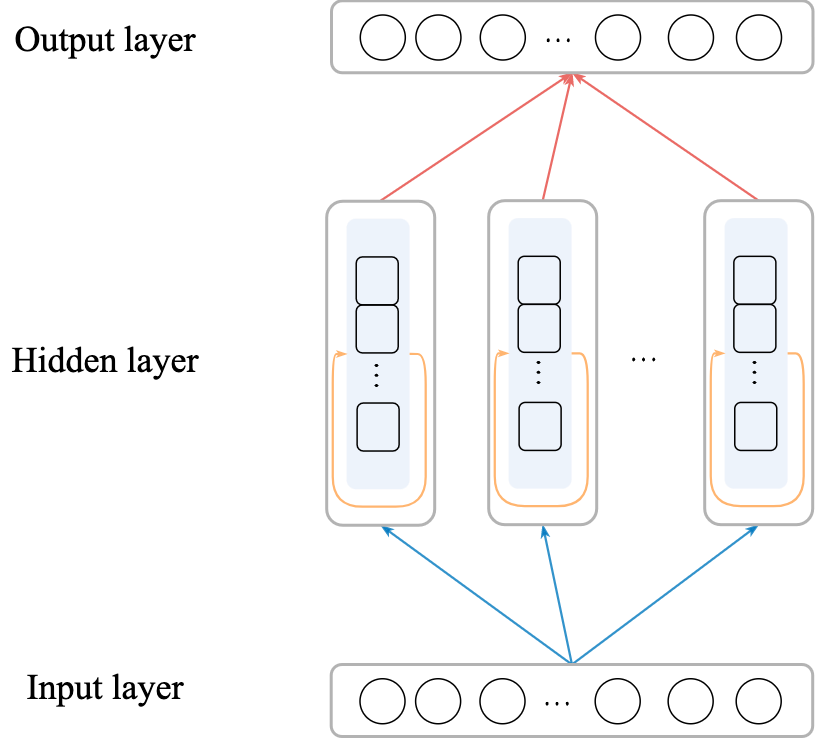
\includegraphics[height=3cm]{float/ch.intro/gesn.png}%
            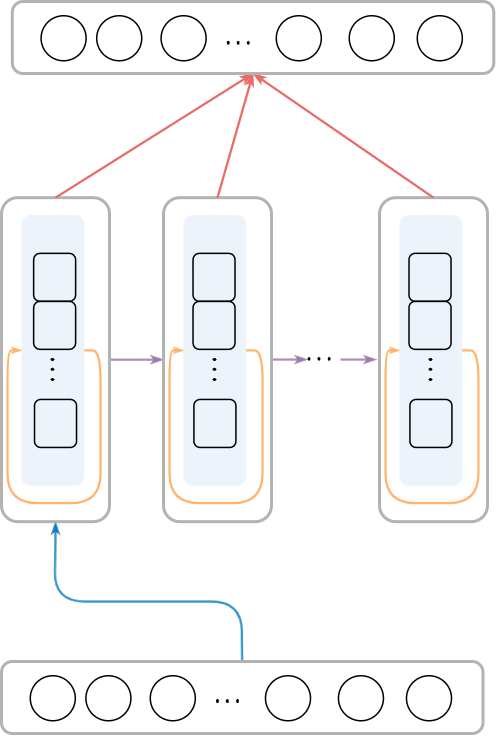
\includegraphics[height=3cm]{float/ch.intro/desn.png}%
        }%
    }
    \setlength{\twosubht}{\ht\twosubbox}    
    \centering
    \subcaptionbox{\label{fig:ch.intro.gesn}GESN结构}{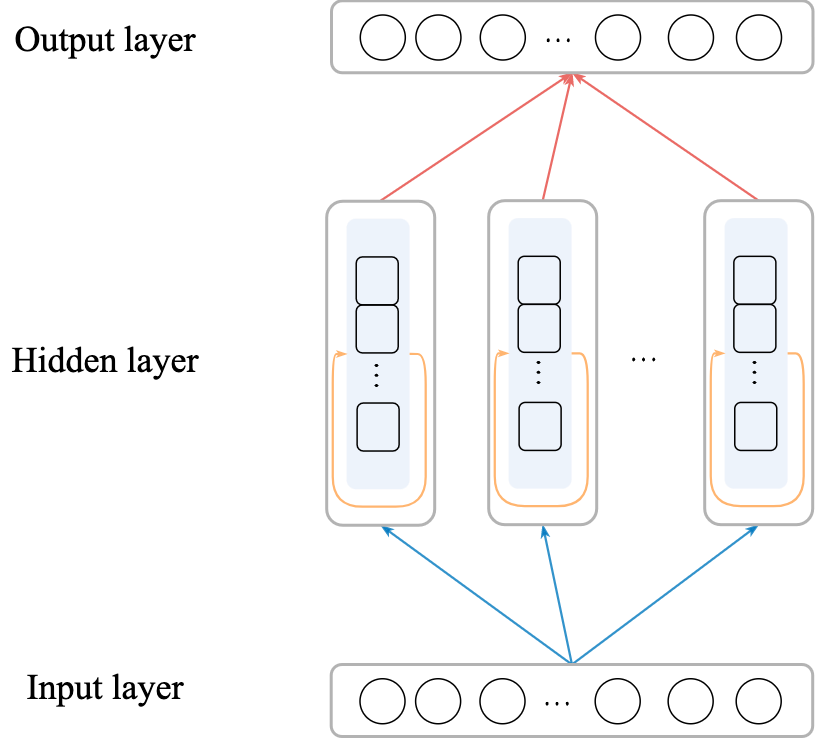
\includegraphics[height = \twosubht]{float/ch.intro/gesn.png}}
    \quad
    \subcaptionbox{\label{fig:ch.intro.desn}DESN结构}{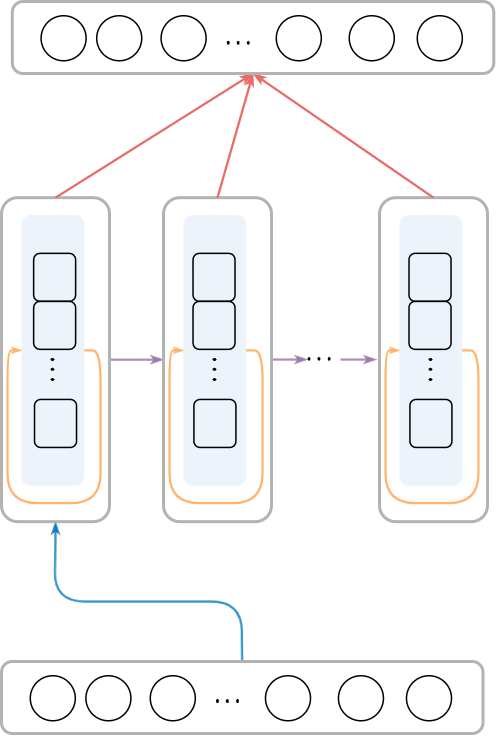
\includegraphics[height = \twosubht]{float/ch.intro/desn.png}}
    \caption{\label{fig:ch.intro.esns} GESN与DESN结构示例}
\end{figure*}

相比循环结构的SDNN预测建模技术研究,基于卷积结构的SDNN预测建模研究则更为薄弱 。He et al.~\cite{hePowerful2016}首先发现了基于随机卷积核的VGG构型\footnote{{https://www.robots.ox.ac.uk/~vgg/research/very\_deep/}}~\cite{simonyanVery2015}CNN在纹理生成(Texture synthesis)和风格迁移(Style transfer)等任务上具有不亚于梯度下降训练CNN的表现。受此启发,Antognini et al.~\cite{antogniniAudio2019}发现了基于一维卷积结构的随机CNN模型在音频纹理生成任务上同样可以达到与训练CNN一样的性能。进一步地,Yu et al.~\cite{yuImpact2019}在合成时间序列数据集和煤气供应数据集等现实时间序列数据集上进行了一维随机CNN的预测建模实验,展示了随机映射方法在CNN预测建模技术中的可行性。

由此,针对时间序列深度学习预测技术模型选择挑战中的低效问题,构造基于随机映射的深度学习预测建模技术是一种有效的解决途径,既可以兼具深度学习建模技术优异的预测潜能,又可以利用随机映射技术收敛快、效率高的优势,从而高效灵活的解决深度学习预测建模技术的模型选择效率问题,为时间序列深度学习预测建模技术的实际应用和发展提供支撑。

然而,基于随机映射方法的预测建模研究,尤其是SDNN预测建模研究,仍有一些突出的问题和限制。这些问题对于不同的神经网络结构,如卷积结构和循环结构,呈现出不同的复杂表现。
例如,相较于梯度下降方法,随机映射方法在提升模型建模效率的同时,因其输入层和隐藏层权重参数的随机性,不可避免地在一定程度上降低了模型的预测性能,这种现象对于具备复杂表征结构的卷积结构SDNN预测模型而言尤为突出,如何设计一种卷积结构SDNN预测模型构造与选择方法以保持模型建模效率与预测性能的平衡性是基于卷积结构的SDNN预测建模技术研究中的重要问题。

又如,现有循环结构SDNN预测模型(即ESN预测模型)的研究主要集中于隐藏神经网络结构的设计与优化\cite{liPSObased2019,chouikhiPSObased2017},而输出结构选择问题尚未有关注。在ESN预测模型的输出结构设计中,存在诸多问题,如基于梯度下降方法所构造的RNN模型输出结构是否适用于随机映射方法下的循环结构建模技术和方法,这些输出结构对于ESN模型输出结构的优化有何启示,如何选择与优化ESN预测模型的循环输出结构等。这些问题是基于循环结构的SDNN预测建模技术研究中的重要问题,需要进一步研究和探索。

再者,时间序列输入特征的选择问题是以CNN与RNN为代表的不同结构DNN预测建模技术共性问题,如何将深度神经网络结构与时间序列输入特征有效结合,从而建立兼容不同结构SDNN预测模型的特征选择方法,是进一步系统提升SDNN预测模型性能的关键。

此外,基于不同结构的SDNN预测建模有着不同的特性和适用场景。单一特定结构下的SDNN预测建模与优化方法难以适应复杂多变的现实时间序列预测需要。如何集成多种深度神经网络结构的优势,针对不同的时间序列预测建模场景,自适应地选择合适的神经网络结构及其参数,从而建立SDNN预测模型混合结构下的构造与优化技术,亦是基于随机映射的深度学习预测建模技术研究及其应用中的关键问题。

因此,为解决现有深度学习预测建模技术与随机映射方法的不足,本文将在时间序列深度学习预测建模技术与随机映射方法相关研究的基础上,尝试设计SDNN预测模型的新颖构造方法,以消除传统迭代训练的DNN预测模型所带来的低效性问题和随机映射方法在DNN网络结构上的不稳定性,同时建立与预测问题和预测模型相适应的模型选择算法,
探索具备高效自适性、理论创新性和良好应用性的SDNN时间序列建模技术。
本研究在一定程度上推动深度学习预测模型理论发展,充分挖掘随机映射方法在时间序列深度学习预测建模技术中的性能潜力,具有一定的理论创新意义和良好的现实应用意义。
